% The command below calls the preprint style^M
% which will produce a one-column, single-spaced document.^M
% Examples of commands for other sub-styles follow. Use^M
% whichever is most appropriate for your purposes.^M

%\documentclass[12pt,preprint]{aastex}
%\documentclass[iop,appendixfloats]{emulateapj}

% manuscript produces a one-column, double-spaced document:

%\documentclass[manuscript]{aastex}
%----------------------------------
% mn2esample.tex
%
% v2.1 released 22nd May 2002 (G. Hutton)
%
% The mnsample.tex file has been amended to highlight
% the proper use of LaTeX2e code with the class file
% and using natbib cross-referencing. These changes
% do not reflect the original paper by A. V. Raveendran.
%
% Previous versions of this sample document were
% compatible with the LaTeX 2.09 style file mn.sty
% v1.2 released 5th September 1994 (M. Reed)
% v1.1 released 18th July 1994
% v1.0 released 28th January 1994

\documentclass[useAMS,usenatbib,letters]{mn2e}

% If your system does not have the AMS fonts version 2.0 installed, then
% remove the useAMS option.
%
% useAMS allows you to obtain upright Greek characters.
% e.g. \umu, \upi etc.  See the section on "Upright Greek characters" in
% this guide for further information.
%
% If you are using AMS 2.0 fonts, bold math letters/symbols are available
% at a larger range of sizes for NFSS release 1 and 2 (using \boldmath or
% preferably \bmath).
%
% The usenatbib command allows the use of Patrick Daly's natbib.sty for
% cross-referencing.
%
% If you wish to typeset the paper in Times font (if you do not have the
% PostScript Type 1 Computer Modern fonts you will need to do this to get
% smoother fonts in a PDF file) then uncomment the next line
% \usepackage{Times}

%%%%% AUTHORS - PLACE YOUR OWN MACROS HERE %%%%%
\usepackage{color}
\usepackage{graphicx}
\usepackage{amsmath}
\usepackage{amssymb}
\definecolor{orange}{rgb}{1,0.5,0}
\usepackage[colorlinks=True,citecolor=orange,urlcolor=blue,linkcolor=red]{hyperref}

\newcommand{\figurepath}{.}


%  Definition of fonts


\newcommand{\tom}{\tilde{\omega}}

\newcommand{\ri}{r_{\rm i}}

\newcommand{\ro}{r_{\rm out}}

\newcommand{\rs}{r_{\star}}

\newcommand{\mj}{\dot{M}_{\rm jet}}

\newcommand{\ms}{\dot{M}_{\star}}

\newcommand{\vk}{v_{\rm K}}

\newcommand{\ti}{t_{\rm i}}

\newcommand{\rj}{R_{\rm jet}}

\newcommand{\rk}{R_{\kappa}}

\newcommand{\cs}{c_{\rm s}}

\newcommand{\css}{c_{\rm s}^2}

\newcommand{\bp}{B_{\rm P}}

\newcommand{\bh}{B_{\phi}}

\newcommand{\jp}{\vec{B}_{\rm P}}

\newcommand{\cm}{{\rm cm}}

\newcommand{\msun}{{\rm M}_{\sun}}

\newcommand{\rsun}{{\rm R}_{\sun}}

\newcommand{\rstar}{{\rm R}_{\star}}

\newcommand{\lumsun}{{\rm L}_{\sun}}

\newcommand{\lumstar}{{\rm L}_{\star}}

\newcommand{\lumdisk}{{\rm L}_{\rm disk}}

\newcommand{\etat}{{\eta}_{\rm t}}

\newcommand{\betat}{{\beta}_{\rm t}}

\newcommand{\betai}{{\beta}_{\rm i}}

\newcommand{\deltai}{{\delta}_{\rm i}}

\newcommand{\rhoi}{{\rho}_{\rm i}}

% Bibliography and bibfile
\def\aj{AJ}%
          % Astronomical Journal
\def\actaa{Acta Astron.}%
          % Acta Astronomica
\def\araa{ARA\&A}%
          % Annual Review of Astron and Astrophys
\def\apj{ApJ}%
          % Astrophysical Journal
\def\apjl{ApJ}%
          % Astrophysical Journal, Letters
\def\apjs{ApJS}%
          % Astrophysical Journal, Supplement
\def\ao{Appl.~Opt.}%
          % Applied Optics
\def\apss{Ap\&SS}%
          % Astrophysics and Space Science
\def\aap{A\&A}%
          % Astronomy and Astrophysics
\def\aapr{A\&A~Rev.}%
          % Astronomy and Astrophysics Reviews
\def\aaps{A\&AS}%
          % Astronomy and Astrophysics, Supplement
\def\azh{AZh}%
          % Astronomicheskii Zhurnal
\def\baas{BAAS}%
          % Bulletin of the AAS
\def\bac{Bull. astr. Inst. Czechosl.}%
          % Bulletin of the Astronomical Institutes of Czechoslovakia 
\def\caa{Chinese Astron. Astrophys.}%
          % Chinese Astronomy and Astrophysics
\def\cjaa{Chinese J. Astron. Astrophys.}%
          % Chinese Journal of Astronomy and Astrophysics
\def\icarus{Icarus}%
          % Icarus
\def\jcap{J. Cosmology Astropart. Phys.}%
          % Journal of Cosmology and Astroparticle Physics
\def\jrasc{JRASC}%
          % Journal of the RAS of Canada
\def\mnras{MNRAS}%
          % Monthly Notices of the RAS
\def\memras{MmRAS}%
          % Memoirs of the RAS
\def\na{New A}%
          % New Astronomy
\def\nar{New A Rev.}%
          % New Astronomy Review
\def\pasa{PASA}%
          % Publications of the Astron. Soc. of Australia
\def\pra{Phys.~Rev.~A}%
          % Physical Review A: General Physics
\def\prb{Phys.~Rev.~B}%
          % Physical Review B: Solid State
\def\prc{Phys.~Rev.~C}%
          % Physical Review C
\def\prd{Phys.~Rev.~D}%
          % Physical Review D
\def\pre{Phys.~Rev.~E}%
          % Physical Review E
\def\prl{Phys.~Rev.~Lett.}%
          % Physical Review Letters
\def\pasp{PASP}%
          % Publications of the ASP
\def\pasj{PASJ}%
          % Publications of the ASJ
\def\qjras{QJRAS}%
          % Quarterly Journal of the RAS
\def\rmxaa{Rev. Mexicana Astron. Astrofis.}%
          % Revista Mexicana de Astronomia y Astrofisica
\def\skytel{S\&T}%
          % Sky and Telescope
\def\solphys{Sol.~Phys.}%
          % Solar Physics
\def\sovast{Soviet~Ast.}%
          % Soviet Astronomy
\def\ssr{Space~Sci.~Rev.}%
          % Space Science Reviews
\def\zap{ZAp}%
          % Zeitschrift fuer Astrophysik
\def\nat{Nature}%
          % Nature
\def\iaucirc{IAU~Circ.}%
          % IAU Cirulars
\def\aplett{Astrophys.~Lett.}%
          % Astrophysics Letters
\def\apspr{Astrophys.~Space~Phys.~Res.}%
          % Astrophysics Space Physics Research
\def\bain{Bull.~Astron.~Inst.~Netherlands}%
          % Bulletin Astronomical Institute of the Netherlands
\def\fcp{Fund.~Cosmic~Phys.}%
          % Fundamental Cosmic Physics
\def\gca{Geochim.~Cosmochim.~Acta}%
          % Geochimica Cosmochimica Acta
\def\grl{Geophys.~Res.~Lett.}%
          % Geophysics Research Letters
\def\jcp{J.~Chem.~Phys.}%
          % Journal of Chemical Physics
\def\jgr{J.~Geophys.~Res.}%
          % Journal of Geophysics Research
\def\jqsrt{J.~Quant.~Spec.~Radiat.~Transf.}%
          % Journal of Quantitiative Spectroscopy and Radiative Trasfer
\def\memsai{Mem.~Soc.~Astron.~Italiana}%
          % Mem. Societa Astronomica Italiana
\def\nphysa{Nucl.~Phys.~A}%
          % Nuclear Physics A
\def\physrep{Phys.~Rep.}%
          % Physics Reports
\def\physscr{Phys.~Scr}%
          % Physica Scripta
\def\planss{Planet.~Space~Sci.}%
          % Planetary Space Science
\def\procspie{Proc.~SPIE}%
          % Proceedings of the SPIE
\let\astap=\aap
\let\apjlett=\apjl
\let\apjsupp=\apjs
\let\applopt=\ao

\newcommand{\figpath}{PFIGS/}
%%%%%%%%%%%%%%%%%%%%%%%%%%%%%%%%%%%%%%%%%%%%%%%%

\begin{document}
\title{SiO Molecular Jets around young stars - A numerical perspective}
\author[B. Vaidya, Tom Douglas, Paola Caselli, Tom Hartquist]{B. Vaidya$^{1}$\thanks{E-mail:
B.Vaidya@leeds.ac.uk (BV)}, Tom Douglas$^{1}$, Paola Caselli$^{1}$, Tom Hartquist$^{1}$\\
$^{1}$School of Physics and Astronomy, University of Leeds, Leeds LS2
9JT\\
}

\date\today

%\date{Accepted yyyy m dd. Received yyyy m dd; in original yyyy m dd}
\pagerange{\pageref{firstpage}--\pageref{lastpage}} \pubyear{yyyy}


\maketitle

\label{firstpage}

\begin{abstract}
  % context heading (optional)
  {}  
  % aims heading (mandatory)
   {}
  % methods heading (mandatory)
   {}
  % results heading (mandatory)
   {}
  % conclusions heading (optional), leave it empty if necessary 
\end{abstract}

   \begin{keywords}
    MHD -- methods:numerical -- ISM: jets and outflows
   \end{keywords}


%
%

%===============================================================

\section{Introduction} 
Interaction of jet with ambient medium , Class 0 sources, momentum and
energy injection, High mass and low mass outflows \\

Observations of Outflows in CO and SiO in mm, H2 in IR, Optical jets
HH objects, syncrotron emission \\

Molecules from jet driven or wind driven, Interesting features like
EHV, low velocity component etc, list interesting outflows from Class 0 \\

Attempts of simulations either only dynamics with analytic approaches
to compare observational features, or only chemistry to estimate
abundances. The reality lies in the middle!\\

Combine dynamics of MHD jet with molecular chemistry and comparing
with observations via post-processing simulations with line radiative
transfer codes. \\

Paper Layout \\

\section{Numerical Setup}
\subsection{Numerical code and Equations}
For our study, we carry out axisymmetric numerical ideal MHD simulations using the PLUTO code \citep{Mignone:2007p644} which is based on a conservative scheme of Godunov type.
We have modified the original code to incorporate molecular cooling
from self-consistent evolution of hydrogen chemistry (see Sect.~\ref{sec:chem}).

  
In general, the MHD code considers the following set of equations.
The conservation of the mass and the momentum,
%
\begin{equation}\label{masscons}
\frac{\partial \rho}{\partial t} + (\vec{v} \cdot \nabla)\rho  +
\rho \nabla \cdot \vec{v} = 0
\end{equation}
%
\begin{equation}\label{momcons}
\rho(\frac{\partial \vec{v}}{\partial t} +
(\vec{v} \cdot \nabla) \vec{v}) =
- \nabla P + \frac{1}{4\pi} (\nabla \times \vec{B}) \times \vec{B}
\end{equation}
%
where $\rho$ is gas density, $\vec{v}$ the velocity vector, $P$ the gas pressure,
and $\vec{B}$ the magnetic field vector with the poloidal and toroidal
components - $\vec{B}_{\rm p}, {B}_{\phi}$. Note that the forces due
to gravity are neglected for this problem as the domain of interest is
far away from the central object (i.e., star).  
%

The cooling function $\Lambda$ which dependents on temperature $T$, mass density $\rho$ and
chemical abundances {\bf{X}}, appears in the
energy equation as a source term,

\begin{equation}\label{encons1}
\frac{\partial}{\partial t}(\rho E)
+ \nabla \cdot\left[ \rho E \vec{v} + (P + \frac{B^2}{8\pi})\vec{v}\right]  
- \vec{B}(\vec{v}\cdot\vec{B}) = \Lambda(\rho,T,{\bf{X}}),
\end{equation}
%
%\begin{equation}\label{encons1}
%\frac{\partial}{\partial t}(\rho {\rm E}) + \nabla.\left[ (\rho
%{\rm E})\textbf{v} + (\textbf{P} + \frac{B^2}{8
%\pi})\textbf{v}\right] - \textbf{B}(\textbf{v.B}) = \rho\left[
%-\nabla\Phi + (\textbf{F}^{\rm rad})\right].\textbf{v}
%\end{equation}
%
where the total energy density of the flow $E$ comprises contributions from 
the internal energy $\epsilon$, the mechanical energy and the magnetic energy,
%
\begin{equation}\label{encons2}
 E = \epsilon + \frac{v^2}{2} + \frac{B^2}{8 \pi \rho}.
\end{equation}
The gas pressure in the flow is related to the density assuming an equation 
of state with the adiabatic index $\gamma$,
%
\begin{equation}\label{EOS}
P = (\gamma - 1) \rho \epsilon.
\end{equation}

The evolution of chemical abundances for each species is solved via,
%
\begin{equation}\label{chemevol}
\frac{\partial \rho{\bf{X}}_{i}}{\partial t} + \nabla \cdot (\rho
{\bf{X}}_{i} \vec{v})  = \rho {\bf{S}}_{i},
\end{equation}
where ${\bf{S}}_{i}$ represents the net creation or destruction of a
given species through chemical reactions (see Sect.~\ref{sec:chem}).

The evolution of the magnetic field is governed by induction equation,
%
\begin{equation}\label{induction}
\frac{\partial \vec{B}}{\partial t} = \nabla \times \left(\vec{v}\times \vec{B}\right).
\end{equation}
%
In addition to the above set of equations the code obeys the condition of divergence-free 
magnetic fields, $\nabla \cdot \vec{B} = 0$, which is numerically achieved by construction 
since using the Powell's eight wave formulation.
\subsection{Initial Condition}
We model the propagation of jet as it interacts with the molecular
cloud core much further from the central object, i.e., $>$ 1000\,AU. 
Further away from the central source, the downward pull of gravity plays a
negligible role and the dynamics of jet is primarily governed by magnetic fields.
The total magnetic field in jet is dominated by the toroidal
component. This is because the poloidal field decays as $z^{-2}$ as
compared to $z^{-1}$ for toroidal field to maintain the force balance ($z$ is the vertical distance from source). 
The hoop stress due to pinch force from toroidal magnetic fields maintains the
a highly collimated beam like structure for the jet.
%

The ambient medium with which the jet interacts primarily
represents the molecular cloud core. The numerical domain is axi-symmetric
and in (r,z,$\phi$) cylindrical co-ordinates. Its extent in radial
direction is 20 $R_{\rm j}$ and 100
$R_{\rm j}$ along the vertical axis, $R_{\rm j}$ being the radius of
the jet. The domain is resolved by an uniform grid with 200 cells in
radial and 1000 cells in vertical direction. For simplicity, we choose this medium
to be unmagnetized and non-turbulent. The density in the ambient
medium varies with vertical height $z$ as, $\rho_{\rm amb}\sim (\rho_0/z^{2})$
consistent with observations \citep{Caselli:2011p13935}. The value of
$\rho_0$ depends upon the density contrast, $\eta$, between the jet and
the ambient medium. The number density in the jet is kept fixed such
that the density in ambient medium lies within a range of $10^{4}-10^{5}
\rm cm^{-3}$. The pressure in the ambient molecular medium is
set so to maintain a constant temperature of 50\,K. 
%

The jet enters into the medium through a nozzle of radius $R_{\rm jet}$
from the lower boundary (z = 0). The jet density is fixed to
be $10^{5} \rm cm^{-3}$ and it has a radius of $2.5\times10^{15} \rm cm \sim
167\,AU$. The jet is injected into the domain with a typical 
velocity of $v_{\rm jet,0}$ = 100 km/s as is the case for most low mass stellar jets
specially the low velocity component. The constant jet velocity is
superimposed with periodic pulsation of the form,
\begin{equation}
v_{\rm jet} = v_{\rm jet,0}(1.0 + A\,sin(2.0\pi t/T_{\rm p}))
\end{equation}
where the amplitude A is 0.25 and time period $T_{\rm p} = 70$
years. The pressure at the surface of the jet is $10^{-10} \rm
dyne\,\,cm^{-2}$ corresponding to a temperature of $T_{\rm jet} \sim
4\times10^{3}\,K$. Inside the jet beam, a radial variation of thermal
and magnetic pressure is adopted to maintain a magneto-static
equilibrium. We adopt the
same radial profiles used by \cite{Stone:2000p2650} for all our runs. 
Based on these profiles, the toroidal magnetic field is assumed to be
zero at the axis and achieves a maximum at some radius, $r_{\rm m}$
inside the jet. The maximum value, $B_{\phi,\rm m}$, depends on the
plasma $\beta$ which is a parameter used for our study along with the
density contrast $\eta$.
%

In order to consistently model the SiO emission arising from shocks as
this jet interacts with the medium, we evolve the dynamics along with
chemistry and cooling prescribtions. They are described in details in
the next section.






 

\section{Chemistry and Cooling}
\label{sec:chem}
\subsection{Power law cooling}
\subsection{Atomic Cooling}
\subsection{Tabulated Cooling}


\subsection{Molecular Cooling}
\label{ssec:molcool}
The evolution of molecular, atomic and ionized hydrogen is governed by
equations listed in Table~\ref{tab:chemeq}. In this cooling mode,
these equations are evolved at each times using temperature dependent
rates mentioned in the table along with their source. The code tracks
the formation and destruction of three quantities viz., X(HI), X($H_{2}$)
and X(HII) with a constraint that sum of all three should be unity.
Further, these abundances are used to update the cooling
function $\Lambda(n,T,{\bf{X}})$ to consistently derive the
temperature for next advection step.


\begin{figure*}
 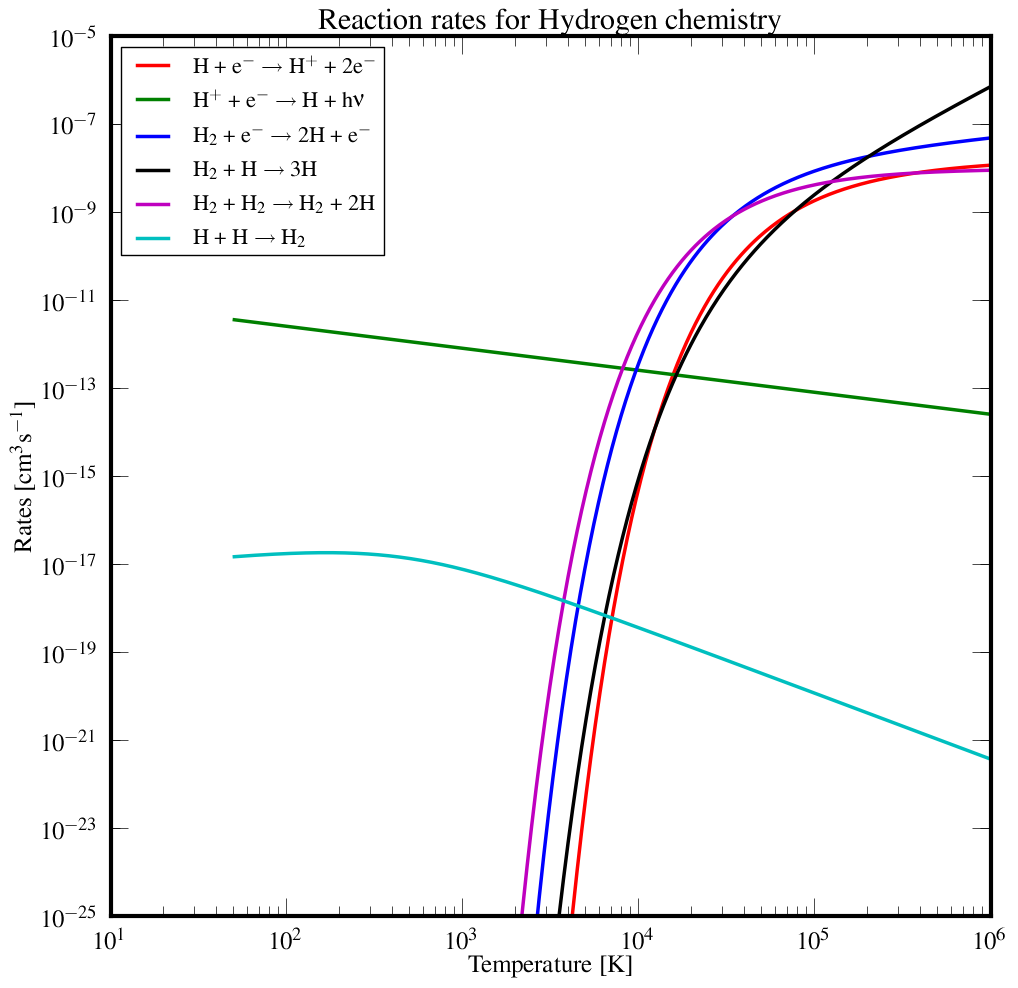
\includegraphics[width=1\columnwidth]{\figpath/H2ReactionRates.png}
 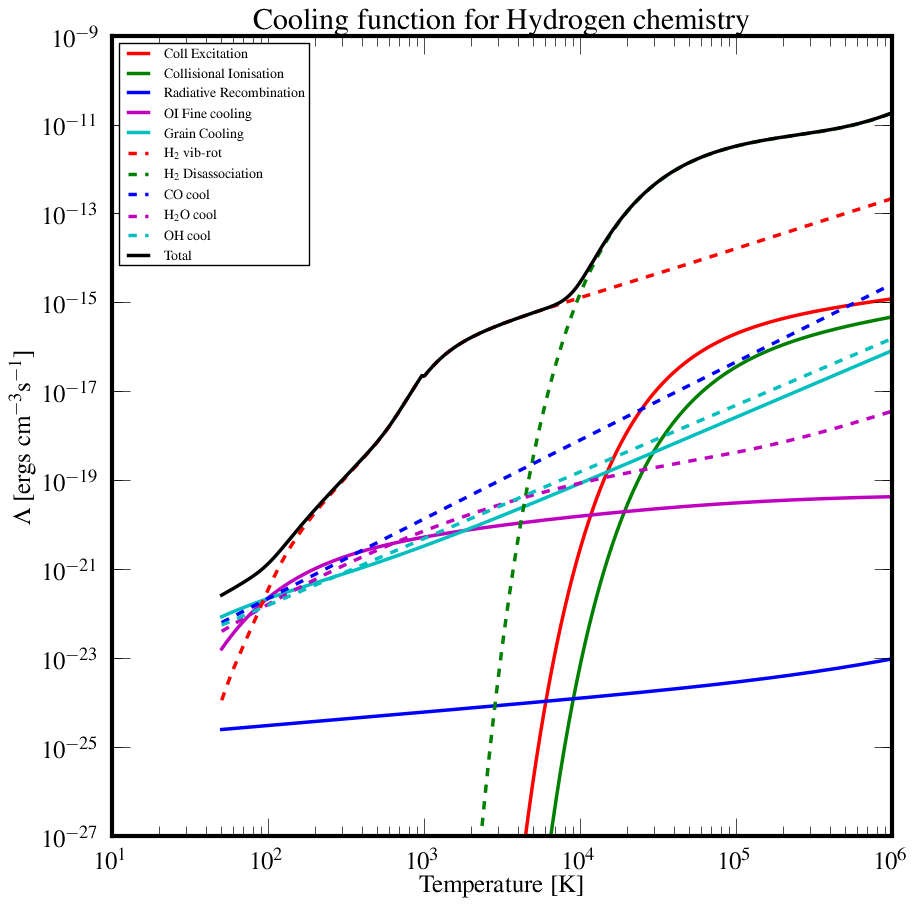
\includegraphics[width=1\columnwidth]{\figpath/H2CoolingFuncs.png}
 \caption{Variation of $H_2$ chemistry reaction rates, $k_{i}$ and cooling
   function $\Lambda(n,T,{\bf{X}})$ with temperature for the initial
   state (see Sect.~\ref{ssec:molcool})}
\label{fig:tempvar}
\end{figure*}

\begin{table*}
\begin{minipage}{\textwidth}
\caption{Summary of the chemistry reaction set. T is the temperature
  in Kelvin, $T_{\rm eV}$ is the temperature in electron-volts, $T_{5}$
  = $T/1\times10^{5}$  and 
$T_{2}$  = T/100}
\label{tab:chemeq}
\begin{tabular}{l l l l}
\hline
No. & Reaction & Rate Coefficient ($\rm {cm}^{3} s^{-1}$) &
Reference~\footnote{REFERENCES -- (1) \cite{Cen:1992p13616} [Eq. 26a];
  (2) \cite{Woodall:2007p13623} [UMIST Database] (3)
  \cite{Galli:1998p13066} [Eq. H17]; (4) \cite{Abel:1997p12836}
  [Tab. 3 Eq. 13]; (5) \cite{Hollenbach:1979p12707} [Eq. 3.8]}\\
\hline
1. & H + e$^{-}$ $\rightarrow$ H$^{+}$ + 2e$^{-}$ & $k_1$ = $5.85
\times 10^{-11}$ $T^{0.5}$ \rm{exp}(-157,809.1/T)/(1.0 + $T_{5}^{0.5}$) & 1\\
2. & H$^{+}$ + e$^{-}$ $\rightarrow$ H + h$\nu$ & $k_2$ =
$3.5\times10^{-12} (T/300.0)^{-0.8}$ & 2\\
3. & H$_{2}$ + e$^{-}$ $\rightarrow$ 2H + e$^{-}$ & $k_3$ =
$4.4\times10^{-10} T^{0.35} \rm{exp}(-102,000.0/T)$ & 3\\
4. & H$_{2}$ + H $\rightarrow$ 3H & $k_4$ = $1.067\times10^{-10}
T_{\rm eV}^{2.012}(\rm{exp}(4.463/T_{\rm eV})^{-1}((1. + 0.2472 T_{\rm eV})^{3.512})^{-1} $& 4\\
5. &H$_{2}$ + H$_{2}$ $\rightarrow$ H$_{2}$ + 2H & $k_5$ = $1.0\times 10^{-8} \rm{exp}(-84,100/T)$ & 2\\
6. & H + H $\overset{\rm dust}\longrightarrow$ H$_{2}$ & $k_6 =
3.0\times10^{-17}\sqrt{T_{2}}(1.0 + 0.4\sqrt{T_{2} + 0.15} + 0.2T_{2} + 0.8T_{2}^{2})$ & 5 \\
\hline
\end{tabular}
\end{minipage}
\end{table*}

\section{Radiative Transfer}
Radiative transfer modeling used for post processing.

\subsection{The radiative transfer code} \label{subsec:radiative_transfer_code}
The radiative transfer program used is LIME (LIne Modeling Engine; \citealt{Brinch:2010p13078}), which  calculates line intensities based on a weighted sample of randomly chosen points in a continuous 3D model. The method of selecting these points is given in section \ref{subsec:gridding}. At each of these points, the density of the main collision partner (equivalent amount of H$_2$, given by n(H$_2$)+ 0.5 n(H)), gas and dust temperatures, velocity, molecular abundances and unresolved turbulent velocity are specified. These points are then smoothed by Lloyd's algorithm \citep{Lloyd1982} in order to minimise the variation in distance between points whilst keeping the same underlying distribution. These points are then connected by Delaunay triangulation and it is between the points connected by this method that photon are allowed to propagate (fig.~\ref{grid}). The level populations of the selected molecules are calculated at each of these points from collisional and radiative (de)excitation and the local radiation field is calculated. This is repeated 20 times with the populations of each level converging towards a single value. This number of iterations is sufficient for the signal to noise ratio of the level populations (as defined in \citealt{Brinch:2010p13078}) to exceed 1000 for 99\% of the points, ensuring that the simulation has converged on a stable level population. After 20 iterations the model is ray-traced in order to produce synthetic brightness maps. The average of ten separate runs was taken to minimise the artefacts in the output images, resulting from the grid construction (Fig.~\ref{points}).


\begin{figure}
 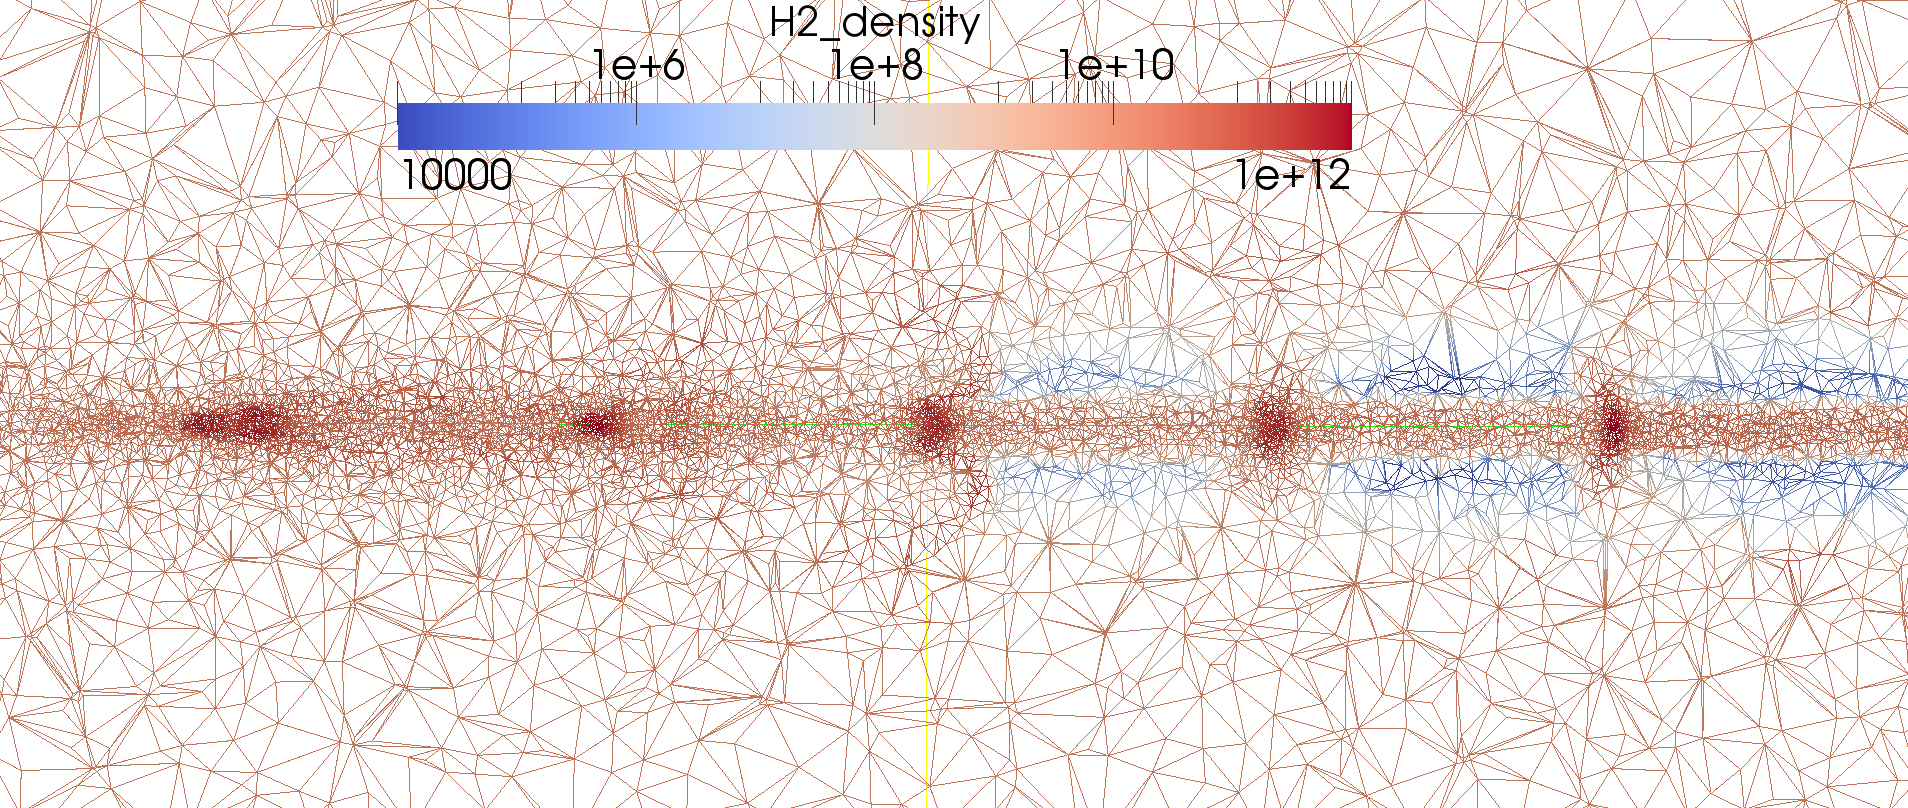
\includegraphics[width=84mm]{\figpath/eta2Beta10.png}
 \caption{A plot of the points selected by the gridding process and the paths down which photons can propagate for points in the r,z plane. The points are color coded by the density distribution (in m$^{-3}$, as used in LIME) and are more concentrated in the high density knots.}
\label{grid}
\end{figure}

\subsection{Grid construction} \label{subsec:gridding}
In order to construct the grid, candidate points are randomly selected from the volume to be simulated. These candidates then have their equivalent H$_2$ number density, and the number density of SiO, compared against those of a reference point in order to decide if the candidate point is to be used in the grid or not. Candidate grid points are selected at random in a cylindrical coordinates that is linearly spaced in z and $\theta$ and logarithmically spaced in r. For each point to be selected, a random number $\alpha$ is drawn from the semi-open set [0,$\,$1) as a threshold. After selection of random coordinates, the H$_2$ density and SiO density at the candidate point (n and m, respectively) are compared against the densities of a reference point in the un-perturbed ambient medium multiplied by $\frac{4\eta}{5}$ (n$_0$ and m$_0$). If $\alpha<\left( \frac{n}{n_0} \right)^{0.3}$ or $\alpha< \left( \frac{m}{m_0} \right)^{0.3}$ then the point is selected for use. Otherwise another r, $\theta$, z co-ordinate is selected and it becomes the candidate point. In addition to this method of selection, 5\% of the points are linearly distributed in x, y and z with no bias with regards to density or abundance. This provides a minimum level of sampling for the large low density regions in the outer parts of the simulated volume. See fig. \ref{points} for an example of the points distribution in r, z. The function comparing the candidate point to the reference point and the candidate point distribution were selected empirically to sample all scales while ensuring that the majority of points are located in the inner disc where the density is higher.  \smallskip

\begin{figure}
 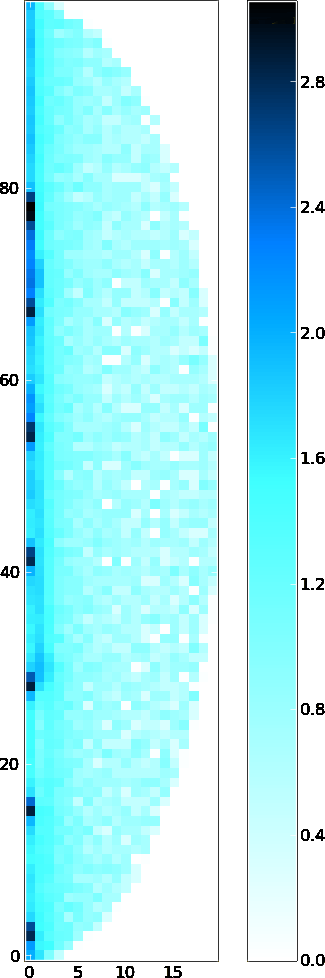
\includegraphics[width=63mm]{\figpath/eta2Beta10_histo.png}
 \caption{A 2D histogram of the point distribution throughout the model. The disc and envelope can be seen as two separate entities which have to be sampled using different point distributions.}
 \label{points}
\end{figure}

\subsection{SiO abundance}
Need refs for this!!\smallskip
The amount of SiO is determined by the local velocity and temperature. The fractional abundance is given by the equation:\smallskip

$log(X)=-2.48\times10^{-8}v^5 + 5.50\times10^{-6}v^4 - 4.28\times10^{-4}v^3 + 1.24\times10^{-2}v^2 + 2.52\times10^{-2}v - 1.20\times10^{1}$\smallskip

where v is in kilometres per second. In addition to this if the temperature at the point is greater than 92,000K (the temperature of the Si-O bond disassociation energy) the abundance is reduced to 10$^{-30}$.

\begin{figure}
 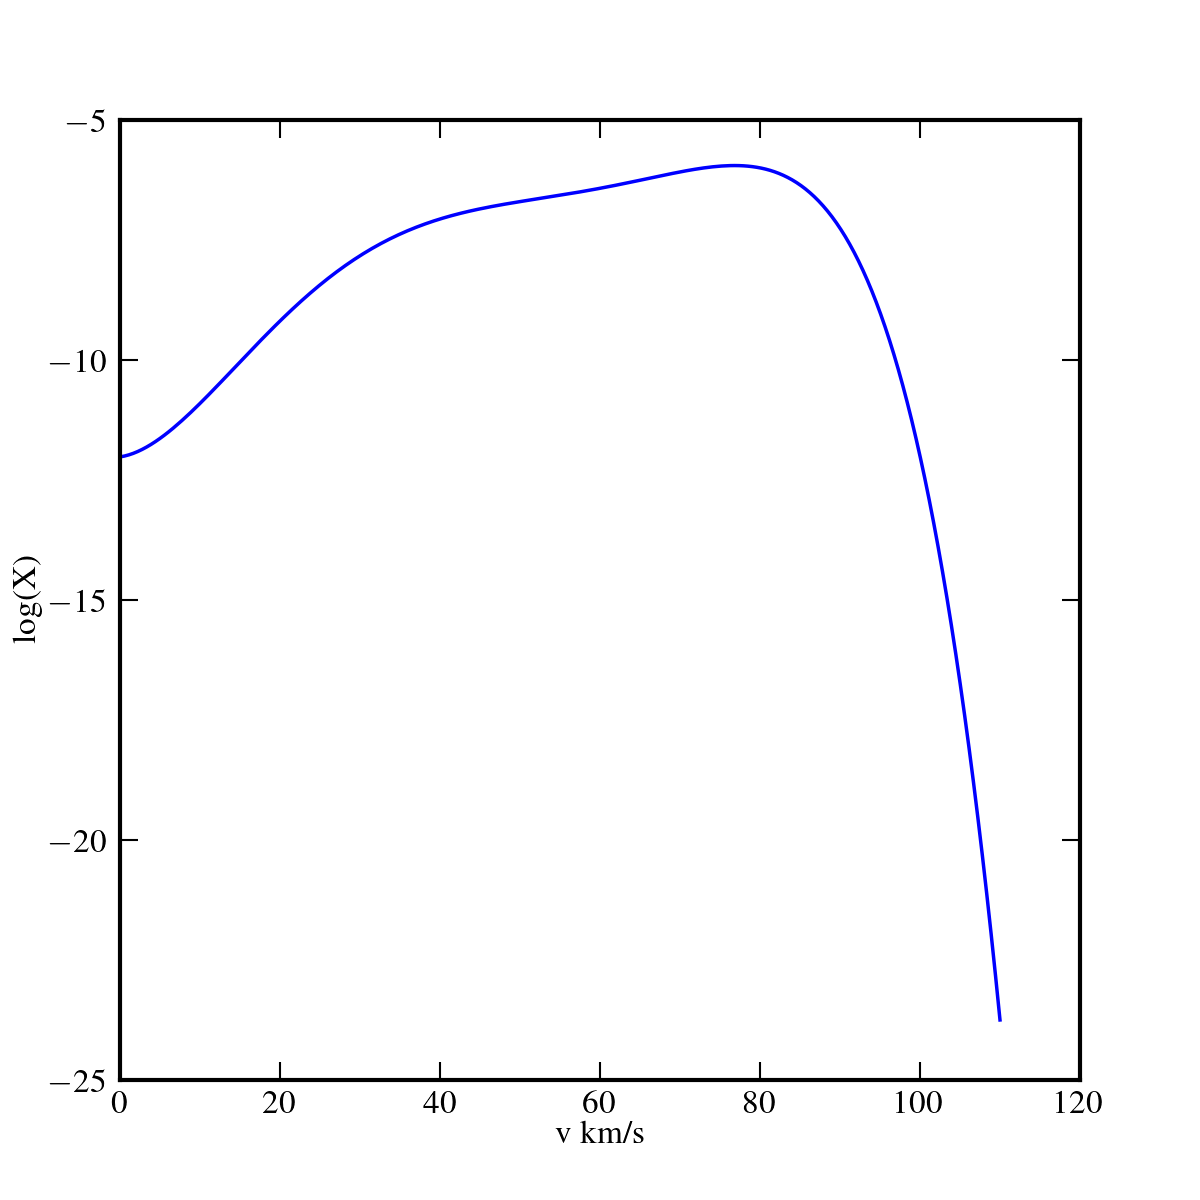
\includegraphics[width=84mm]{\figpath/abun.png}
 \caption{The polynomial used to calculate an abundance of SiO as a function of local velocity.}
 \label{abun}
\end{figure}


\section{Results}
\begin{figure*}
 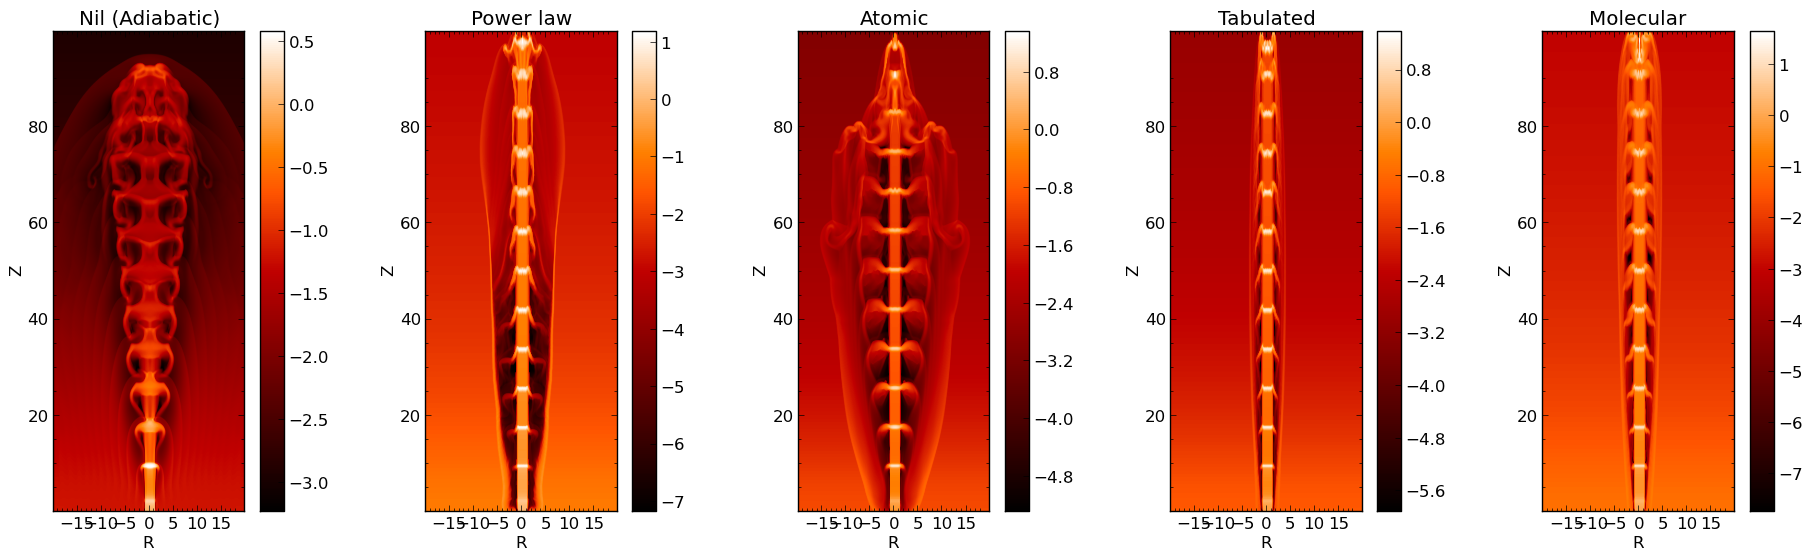
\includegraphics[width=2.\columnwidth]{\figpath/jetplt1_1010.png}
 \caption{Jet Volume Density for different cooling modes with
   $\eta$ = 10 and $\beta$ = 10.}
\label{grid}
\end{figure*}

\section{Results}
\begin{figure*}
 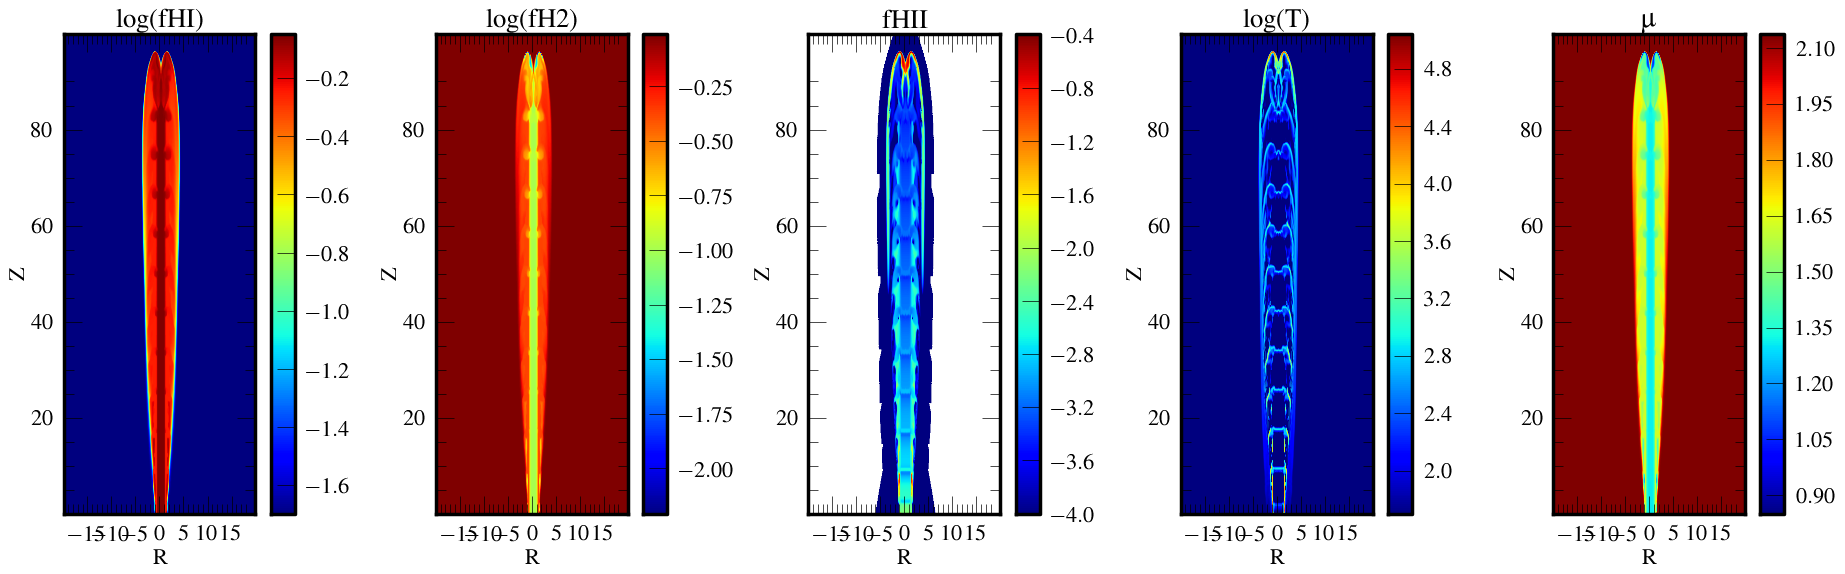
\includegraphics[width=2.\columnwidth]{\figpath/molcjet_510.png}
 \caption{Fraction of hydrogen species in the run with molecular
   cooling having $\eta$ = 5 and $\beta$ = 10.}
\label{grid}
\end{figure*}

\begin{table*}
\centering
\caption{Summary from parameter runs}
\begin{tabular}{l | l | l | l | l | l }
\hline
Run & Cooling Mode & $\eta$ & $\beta$ & Peak Intensity [K] & FWHM at Bow
Shock \\
\hline\hline
adi1010 & Nil (Adiabatic) & 10 & 10 &&\\
pow1010 & Power law & 10 & 10 &&\\
atm1010 & Atomic & 10 & 10 &&\\
atm101 & Atomic & 10 & 1 &&\\
atm210 & Atomic & 2 & 10 &&\\
tab1010 & Tabulated & 10 & 10 &&\\
tab210 & Tabulated & 2 & 10&&\\
mol1010 & Molecular & 10 & 10&&\\
mol510 & Molecular & 5 & 10&&\\
\hline
\end{tabular}
\label{tab:result1}


\end{table*}


\begin{figure}
 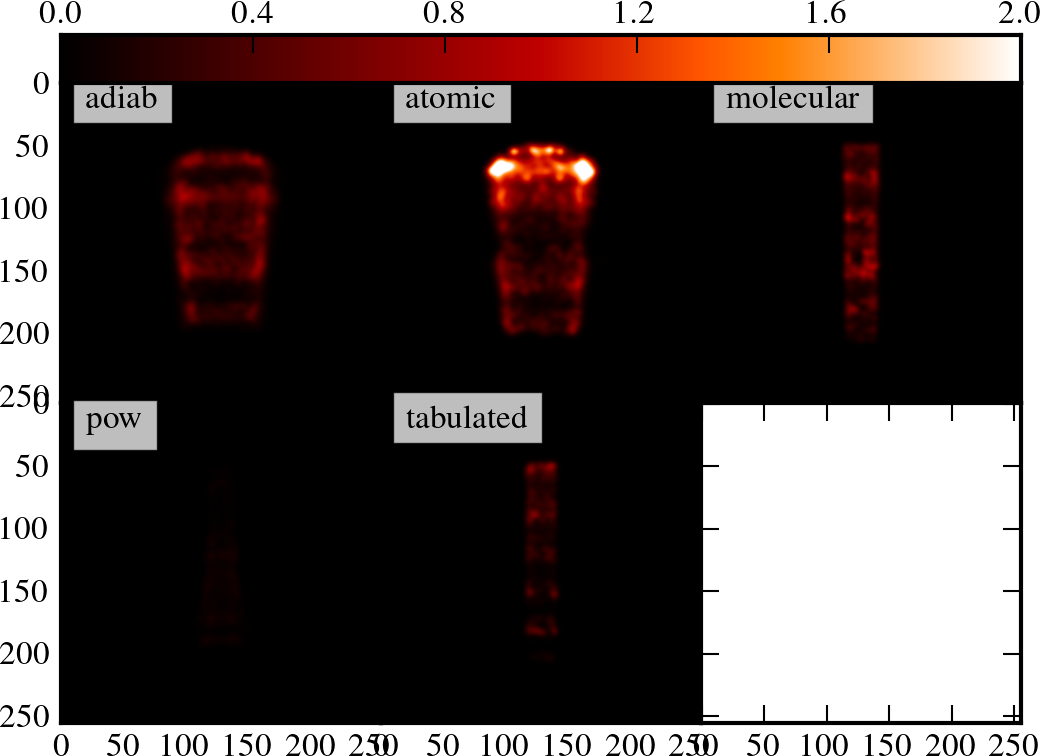
\includegraphics[width=84mm]{\figpath/J2-1_mom0maps_cooling.png}
 \caption{A plot of the integrated SiO J2-1 emission from 5 models, each using a different method to calculate cooling and all with $\eta$=10 $\beta$=10.}
\label{cooling2-1}
\end{figure}

\begin{figure*}
 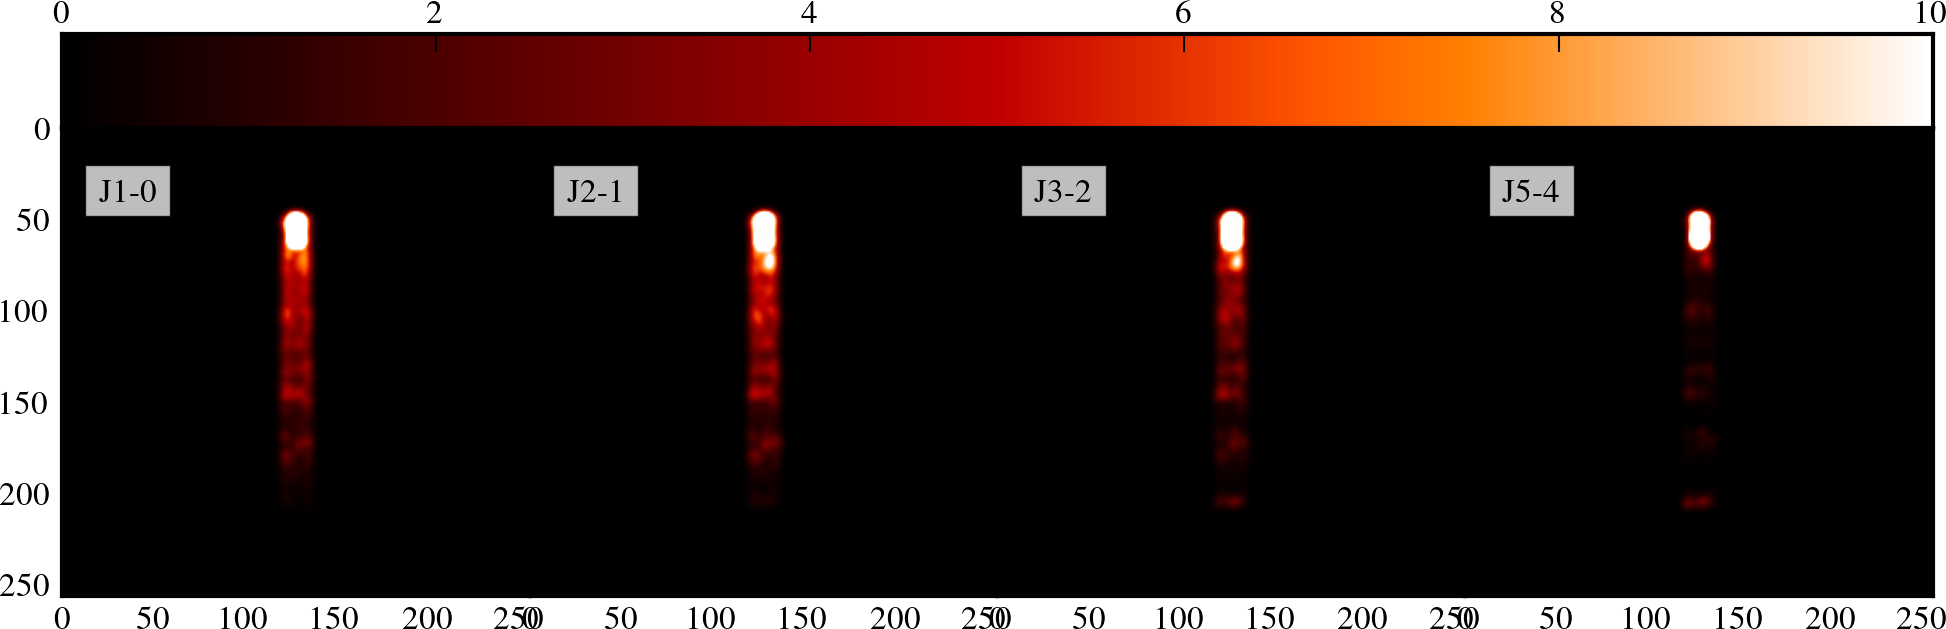
\includegraphics[width=168mm]{\figpath/tabulated_mom0maps_Trans.png}
 \caption{The integrated intensity of 4 SiO transitions in the tabulated cooling model in the $\eta$=2 $\beta$=10 model.}
\label{tabulatedTrans}
\end{figure*}

\begin{figure}
 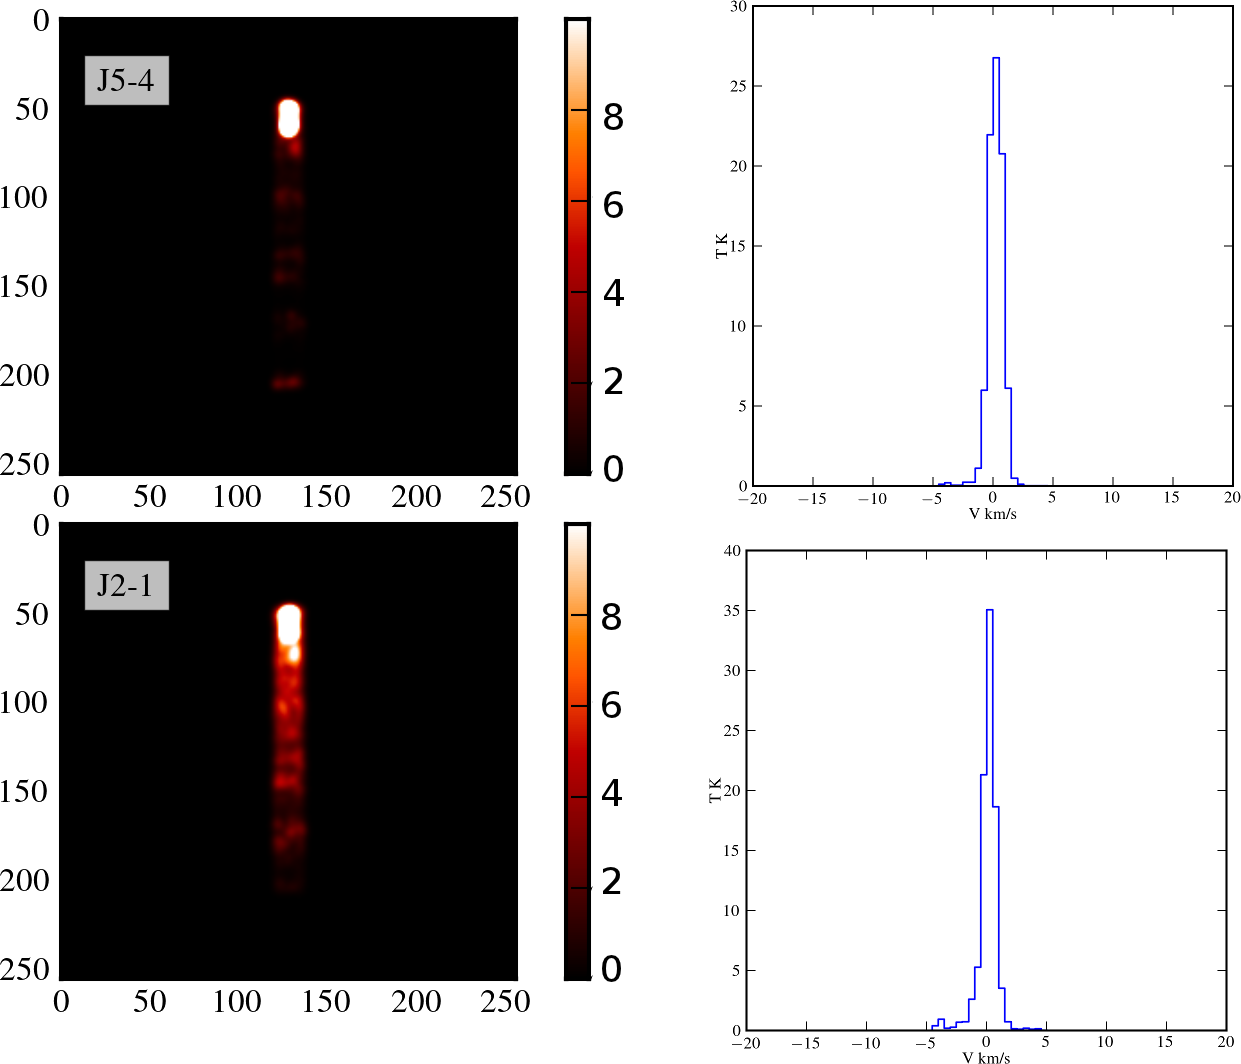
\includegraphics[width=84mm]{\figpath/tab_trans_spectra.png}
 \caption{The Integrated emission and spectra at he bow shock for 2 transitions of the tabulated cooling model for $\eta$=2 $\beta$=10 (spectra taken from y=50, x=128).}
\label{grid}
\end{figure}





Table 1 -- Parameter runs with changing $\beta$ (magnetic fields) and
$\eta$ (density contrast) for cooling \\
Results should have Peak Intensity after convolution., FWHM at tip of
bow shock.\\
Our reference run -- $\beta$ = 10.0, $\eta$ = 2.0, with cooling and
velocity dependent SiO Abundance. \\
Figure 3 -- Output from MHD simulations (Reference run).\\
Figure 4 -- Output from Rad Transfer (Reference run). Integrated
Intensity Maps for different transitions for three different cooling prescribtions. (TODO : TOM)\\
Figure 5 -- Spectra for the reference runs all transitions. (TODO :
TOM)\\
Figure 6 -- PV diagrams (TODO : TOM) for one transition in two directions.
Figure 7 -- Angle of Inclination dependence 
 

\section{Discussion}
Effects of varying $\beta$, $\eta$\\
Importance of cooling prescriptions\\
RADEX plots ratio of Line intensities???\\
Comparison with Observed results \\
Limitations\\

\section{ALMA view}
ALMA view of the reference run and stress of applying our synthetic techniques
to study the molecular outflows in more details.\\
Figure 6. for ALMA -- \\


\section{Conclusion}
We are the best in modelling SiO outflows.



%\section*{Acknowledgments}

\bibliographystyle{mn2e}
\bibliography{bibfile}
\label{lastpage}
\end{document}
